% =========================================================================
\chapter{Introduction}
\label{ch:intro}
% =========================================================================

\claim{A self-evolving harness stalls not for lack of intelligence but for
lack of a readout: we demonstrate a construction mismatch in its evidence column, replace that
evidence with a graph-native record, retype its candidate surface, find
that outcomes do not separate in either direction at the resolution this
bed affords --- measured on three seeds per arm --- and locate the missing
organ, ``did that edit work?'', which none of the systems surveyed here
wires into a retention loop.}

% -------------------------------------------------------------------------
\section{The system under study}
\label{sec:motivation}
% -------------------------------------------------------------------------

An agent is a model plus a harness, and the harness is frequently the
dominant performance lever. That makes the harness a natural target for
automatic optimization, and a literature of self-evolving agents has grown
around the idea~\cite{survey-selfevolve}. Most of it evolves prompts,
workflows or agent code, and by 2026 the harness itself has a line of its
own --- attribution-guided harness repair, gated promotion, harnesses as
editable documents (\S\ref{sec:self-evolving}). What no system in that
line holds is the conjunction this thesis is about: execution provenance,
automated attribution over it, and typed edits written back into a
persisted harness, closed in one loop (\S\ref{sec:positioning}).

HarnessX/AEGIS~\cite{aegis} is one of that line, and is the system this
thesis takes as its object. Its loop runs in six stages. Each round the
solver attempts the bed under a fixed configuration. A \textbf{Digester}
reads every trajectory --- failures and successes alike; the success
template instructs it ``not to celebrate'' but to name the reusable
strategy and any latent fragility --- and writes a per-task dossier. A
\textbf{Planner} synthesizes the dossiers into one landscape. An
\textbf{Evolver} authors zero or more candidate edits to the harness's
configuration, tools, prompt or processors, each as a manifest plus an
applied configuration. A \textbf{Critic} judges each candidate, may
interrogate the Evolver, and audits the candidates as a set against the
scoreboard. Survivors face five deterministic gates, cheapest first ---
structure, novelty, canonicalization, a counterfactual replay over the
previous round's passing tasks, and a synthetic-task smoke --- each
described with what it checks in \S\ref{sec:official-strengths}.
Figure~\ref{fig:official} is the system's own picture of itself;
Figure~\ref{fig:loop} opens its \emph{adapt} vertex into the six stages
just described and marks the seams at which Chapter~\ref{ch:ghx}
attaches.

\begin{figure}[t]
\centering
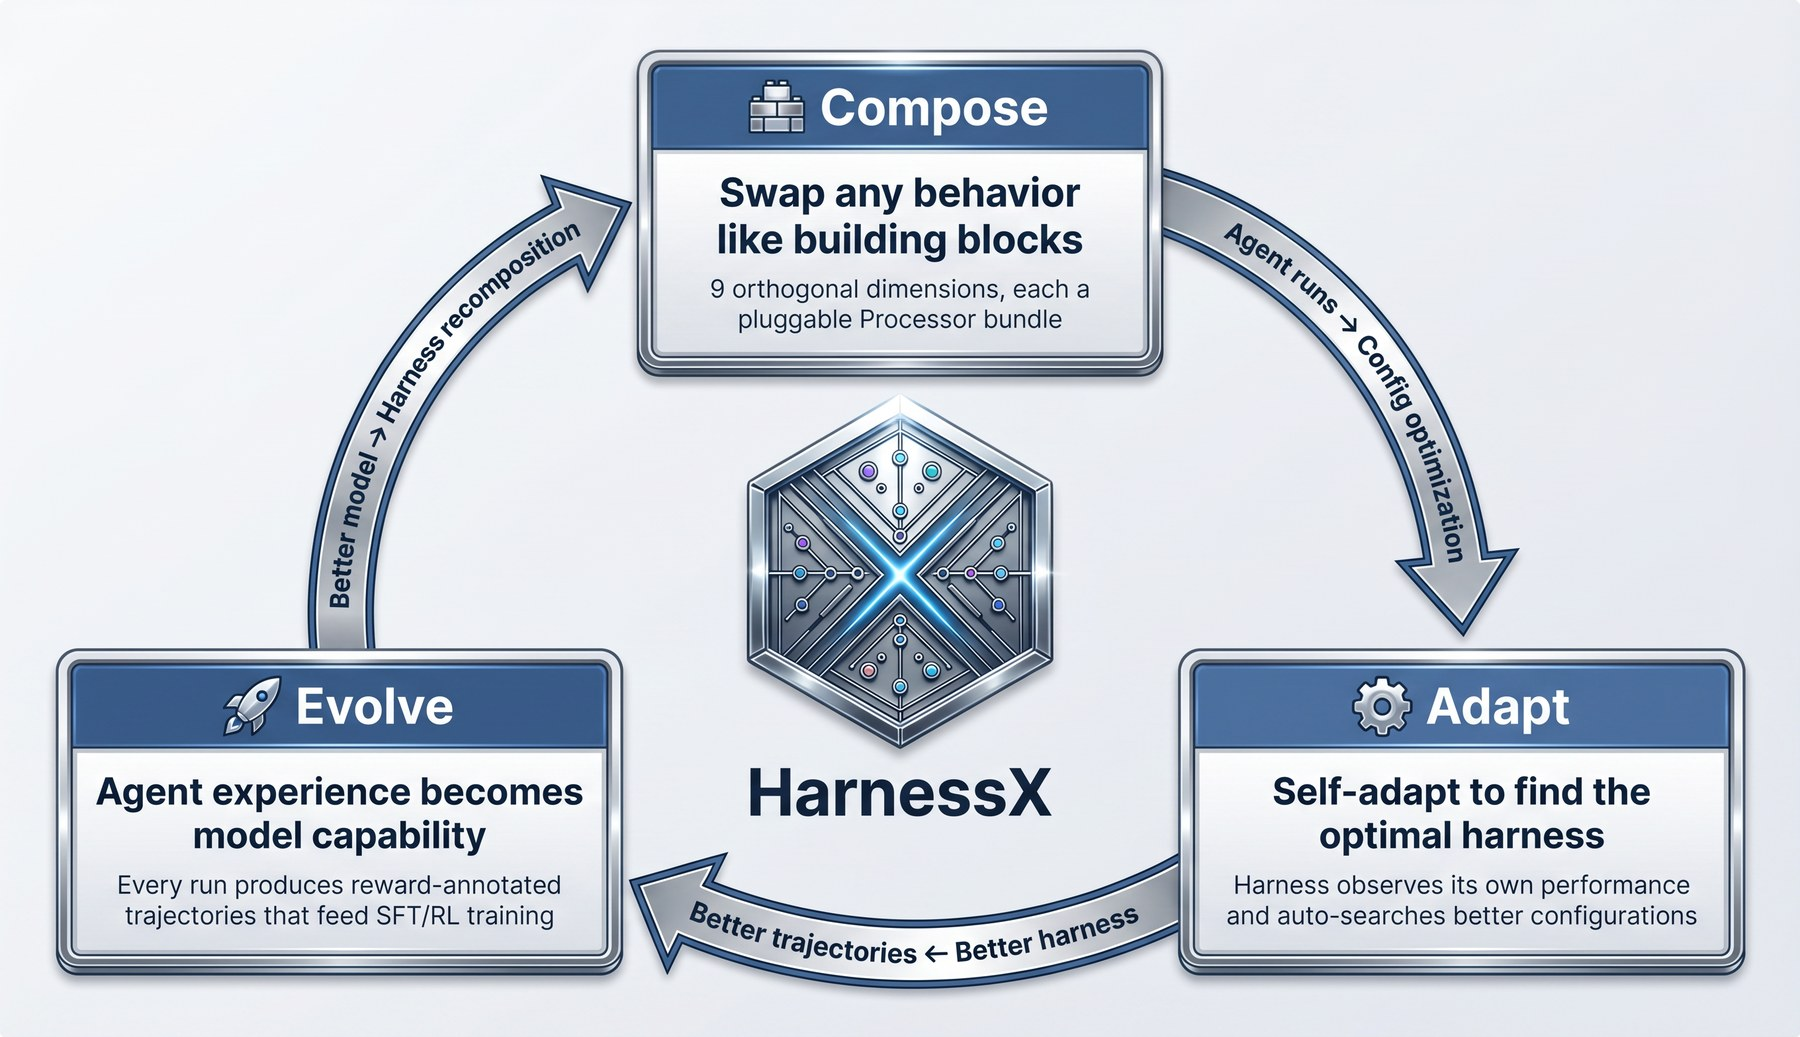
\includegraphics[width=0.88\textwidth]{figures/harnessx_architecture.jpg}
\caption[The official HarnessX overview]{The official system's own
overview of itself: \emph{compose} a harness from pluggable processor
bundles, \emph{adapt} it by letting it observe its own performance and
search better configurations, \emph{evolve} models on the trajectories
it produces. Reproduced from the HarnessX repository's documentation
assets~\cite{aegis} under the repository's MIT licence. The loop this
thesis executes is the \emph{adapt} vertex.}
\label{fig:official}
\end{figure}

That governance is why the system was chosen
as the object of study: a well-guarded loop is the one on which to ask
what the guards can see.

\subsection*{The release against the paper}

The paper's GAIA headline is a $+13.6$-point gain that appears only once
variants are isolated inside an ensemble~\cite{aegis}, and it is the
difference between two peaks rather than a gain over a starting point: the
paper's own single-lineage arm peaks at $73.8\%$ and then \emph{ends at}
$49.5\%$ --- a $24.3$-point collapse its own figure attributes to rollback
failing --- while the ensemble ends at $87.4\%$. No round-zero figure is
published for either \F{68}. The released code is that single lineage: the
variant pool and ensemble routing the headline rests on are absent, leaving
a \texttt{ship\,|\,no\_op} decision on one configuration, the arm whose
published trajectory is the collapsing one.

The headline is therefore not recomputable from the release. What was run
is the released system, not the system the paper describes; the
distinction is maintained throughout, and every divergence between the two
is recorded in Appendix~\ref{app:deviations}.

% -------------------------------------------------------------------------
\section{What was run, and why this bed}
\label{sec:what-was-run}
% -------------------------------------------------------------------------

The system was vendored byte-for-byte under a sha256 manifest enforced by
tests, and executed at scale: six claim-bearing campaigns on the
\textbf{100-task no-pixel bed} drawn from the text-only split of
GAIA~\cite{gaia} --- one bed for every number in this thesis
(\S\ref{sec:beds}).
Each campaign is read over its formal sixteen-round window, so
\textbf{96 rounds and 8{,}393 fresh task evaluations} enter the evidence
base \F{51}. This is an independent execution of the released system.

\subsection*{Why GAIA, and why these hundred tasks}

Four reasons.

\begin{enumerate}
  \item \textbf{It is the authors' bed.} The paper's headline is a GAIA
        number and its own narrative describes a GAIA pilot, so a GAIA bed
        is the one on which the released system can be held to its
        paper.
  \item \textbf{The text-only split keeps the solver inside what the
        recorder can attribute.} GAIA's text-only tasks are answered
        through tools the harness owns --- shell, file reads, web search
        --- so every step of a trajectory is an event the execution graph
        of Chapter~\ref{ch:ghx} can record. Three of the split's 103 tasks
        carry pixel content the recorder cannot attribute; they are
        excluded, which leaves 100. Every number in this thesis is on
        those 100 (\S\ref{sec:beds}).
  \item \textbf{There is room.} Across the six campaigns the union of
        tasks ever solved is 97 of the 100, against a best single round of
        76: twenty-one tasks of headroom that the loop's own history shows
        to be reachable, and 47 tasks that pass sometimes but not
        reliably \F{16}. The bed is neither saturated nor floor-bound.
  \item \textbf{It is small enough to re-run whole, every round.} A
        hundred tasks can be attempted in full sixteen times per campaign,
        which is what makes same-configuration re-measurement
        (Chapter~\ref{ch:design}) affordable.
\end{enumerate}

% -------------------------------------------------------------------------
\section{What running the baseline revealed}
\label{sec:baseline-revealed}
% -------------------------------------------------------------------------

The loop's central evidence signal --- whether a tool call's output was
\emph{used} --- is structurally blind, and the blindness follows from its
own construction.

The column grades a call by whether the immediately next assistant message
shares a verbatim substring of at least twenty characters with the tool
output. GAIA final answers have a median length of nine characters. A short
fact cannot clear that floor however it is used \F{3}.

The remaining baseline observations are null: a flat plateau, an edit
ledger that fixes one thing and breaks another, and shipped-edit margins
inside the same-config re-measurement envelope. This produced the
hypothesis.

\begin{quote}
\textbf{H1.} The loop's failure is an \emph{evidence} problem: faithful
execution-level causal evidence will improve edit localization and
outcomes.
\end{quote}

% -------------------------------------------------------------------------
\section{The hypothesis and its literature}
\label{sec:hypothesis}
% -------------------------------------------------------------------------


H1 was stated as falsifiable, with edit localization as its endpoint. Its
original endpoint proved not measurable on this design, so the original H1
remains untested; the reason that happened is itself the main result
(\S\ref{sec:readout}).

\subsection*{Research questions}
\label{sec:research-questions}

Three questions were posed and all three have settled answers.

\paragraph{Q1, diagnosis.}\label{rq:1} The evidence column has a construction mismatch; the loop's
own \emph{aiming} --- the tasks a candidate names as the ones its edit
will fix --- carries real information within an arm (lift $1.99$, interval
excluding $1.0$ \F{9a}) while the between-arm aiming comparison is not
adjudicable (Q3, \F{9c}); and retention is noise-bounded. Posed from
what running the baseline campaign revealed (\S\ref{sec:baseline-revealed}),
before H1 existed to test.

\paragraph{Q2, non-interference.}\label{rq:2} The recording comparison is
limited to a selected stable cohort; the volatile remainder is not covered
(\S\ref{sec:non-interference}). It therefore supplies a bounded
non-interference observation rather than a whole-bed guarantee.

\paragraph{Q3, the effect of graph evidence.}\label{rq:3} The graph-evidence
effect is not detectable on the available outcome axis, and the original
localization endpoint is not measurable on this design.

% -------------------------------------------------------------------------
\section{GraphHarnessX, in one paragraph}
\label{sec:ghx-preview}
% -------------------------------------------------------------------------

GraphHarnessX --- GHX for the rest of this document --- attaches to the
byte-pinned official substrate from outside and puts the harness and its
execution into one representation. \textbf{The harness itself becomes a
graph}: its executable surface --- hook points, processors, slots, bundles,
skills, tools --- is re-expressed as a typed composition graph which is
then the authority that orders the running pipeline, held to byte-level
parity with the original runloop, and which candidate edits mutate through
typed operations rather than through prose. \textbf{Each invocation of it
becomes a second graph}: an unfolded execution DAG whose data edges are
cross-checked against runtime slot provenance and never invented, carrying
causal ancestor cones (over-approximations of what could have shaped a
failure, never counterfactuals). The pair is what makes rungs R1 and R2 of
\S\ref{sec:readout} mechanical: the composition graph says what a
candidate is and where it sits, the execution DAG says whether it ran and
what it fired on. Four switches are stacked cumulatively --- recording,
then graph evidence, then graph verification, then a typed graph-edit
candidate surface --- each keeping the ones below; the campaigns reported
here fly the whole stack against the stack switched off, not one level at
a time (\S\ref{sec:beds}).

Chapter~\ref{ch:ghx} is the system; Chapter~\ref{ch:design} is how it was
tested.

% -------------------------------------------------------------------------
\section{The verdict of the experiments}
\label{sec:verdict}
% -------------------------------------------------------------------------

Headlines only; every number is in Chapter~\ref{ch:results}.

\begin{itemize}
  \item \textbf{Built and functioning.} The false signal is gone from every
        graph-arm dossier \F{7}; the graph gates have live firing records
        \F{11}; and the loop itself began using the graph \F{38}\F{20}.
  \item \textbf{Outcomes did not separate, in either direction}, at the
        resolution available. Edit localization is \emph{not measurable on
        this design} --- the arms' candidate sets were admitted under
        different gate regimes and drawn against base pools nine points
        apart, which is an absent measurement rather than an underpowered
        null \F{9c}\F{9d}. Scores likewise did not separate: on the common
        bed, arm-mean plateaus differ by $+2.7$ tasks against a between-seed
        standard error of $2.8$ \F{46}, and the within-campaign slope gap
        reaches $p = 0.10$ against a design floor of $0.05$ \F{47}.
        \emph{This is symmetric, and it is not a non-inferiority claim}: no
        margin was pre-specified.
  \item \textbf{One process metric moved, seed-dependently, with its
        mechanism named.} Ship rate across the three graph-arm seeds is
        $0.50$, $0.92$ and $0.60$ per round against a no-graph $0.88$
        \F{10}: two seeds ship below the no-graph figure and one ships
        above it, because the graph arm runs a sixth gate which killed 18
        candidates, pooled over the three graph seeds, that had cleared all
        five official gates for naming a node with no execution record ---
        while the
        share of candidates dying malformed fell by half \F{53}. What
        ships is of higher legality behind one more gate; how many ship
        is not uniformly lower.
  \item \textbf{The candidate surface changed shape}, not reach. Proposals
        became typed graph edits committed atomically with machine-generated
        artifacts, and the loop authored a runtime rule through the
        graph-fed channel that cleared the offline replay gate \F{20}\F{38}.
        The official free-text path could already install a processor, and
        did \F{39}.
  \item \textbf{A pre-specified paired efficacy trial finds no improvement, with a
        negative point estimate}; this is the observed decision-rule result,
        with the mechanism endpoint flat while the treatment engages \F{34}.
\end{itemize}

\paragraph{H1 is not supported, on declared substitute endpoints.} H1 was
stated against edit localization, and localization proved not
measurable here. The archaeology is a descriptive follow-up showing that
the no-graph loop had already prescribed the same drug families correctly,
four campaigns earlier, from $k{=}1$ observations and a
construction-mismatched evidence column \F{38}; the whole-stack two-arm
outcome reading is also descriptive \F{14}\F{46}; and a separately
protocolled efficacy trial reports no improvement, with a negative point
estimate \F{34}. None recovers the original H1 estimand. The endpoint was
substituted after data were seen because the original localization measure
proved unmeasurable; the substitution is reported as a limitation, and the
unmeasurability is itself a result (\S\ref{sec:readout}).

% -------------------------------------------------------------------------
\section{The deeper finding: the missing readout}
\label{sec:readout}
% -------------------------------------------------------------------------

The drug families the evidence-fed loop ``discovered'' had already been
correctly prescribed --- by the official loop, in the zero-graph arm, on
a construction-mismatched evidence column, from single observations, four
campaigns earlier \F{38}. Each family re-surfaces later without
inheriting from the earlier instance: the \textbf{re-prescription
treadmill}.

The axis the loop selects on cannot price such an edit. One intervention
here is known on mechanism grounds to have worked --- a budget-starvation
repair that collapsed a round's budget-exhaustion exits from $35$ to $4$
and moved the score by $+9$ --- and the score axis recovered it, while the
repair then reached no later campaign because the inheritance channel does
not exist \F{39}. Two sweeps over every round pair in every campaign record
the result: \textbf{over the range of effects this loop can produce, the score axis is not a monotone transducer of mechanism magnitude} \F{48}\F{49}.
Score movement is therefore not a monotone proxy for mechanism magnitude,
and a score null remains ambiguous. \S\ref{sec:gain-face} carries the
sweeps and \S\ref{sec:proposition} the conditional argument; the positive
control is a large observed event, not a calibration of smaller effects.

\begin{quote}
\textbf{Self-evolution $=$ variation $+$ selection $+$ readout.}
\end{quote}

The field's selection signal is aggregate score. On this bed it sits below
the noise floor: $21.0$, $20.1$ and $19.2\%$ same-config flips on three
seeds \F{15}\F{9e}, so retention degenerates into drift. The
proposition is about effect detectability under noise, not about
observability of execution; it sits beside, not above, the rival account
that drugs aimed at a capability wall are placebos \F{40}, which
\S\ref{sec:proposition} weighs rather than dismisses. Its constructive
counterpart is a four-rung ladder of evidence about an edit --- \textbf{R0}
in the deployed configuration, \textbf{R1} ever executed ---
answered before landing by replay --- \textbf{R2} fired and on what,
\textbf{R3} did firing change outcomes. The rungs grade
\emph{evidence about an edit}; they are not the cumulative GHX switches of
\S\ref{sec:ghx-preview}, numbered L0--L5 in the run archives, which grade
what the runtime records. R0 to R2 live in GHX \F{11}\F{38}; R3 was built
and exercised by hand here \F{34}\F{36}, and every surveyed system admits
candidates at R0.

% -------------------------------------------------------------------------
\section{Contributions}
\label{sec:contributions}
% -------------------------------------------------------------------------

\begin{description}[leftmargin=3.2em,style=nextline]
  \item[C1] An independent execution and public reading of the official
        self-evolving harness \F{19}\F{51}.
  \item[C2] A quantified audit of its evidence pipeline: a
        \emph{construction} proof that the ``output used'' column cannot
        register the use of a short fact, the rate at which it labels
        answer-carrying calls not referenced, and the reach of that label
        into decisions \F{2}--\F{6} --- established graph-free.
  \item[C3] GHX: a graph-native runtime with non-invasive integration, the
        false signal removed and live gate records \F{7}\F{11}, and a typed,
        transactional candidate surface. \emph{Not} a wider reach --- the
        official Evolver already edits the processor plane, and its one
        above-noise repair was shipped exactly that way \F{39}. The claim
        is \textbf{legality and identity} of candidates \F{20}.
  \item[C4] A diagnosis of H1's unmeasurable original endpoint, together
        with a separately protocolled bundle trial and the measurement
        methodology around it: flip rates, resolution laws, same-window
        paired trials, stopping arithmetic, firing forensics, and a
        fifteen-error registry \F{9c}\F{14}\F{34}\F{38}.
  \item[C5] The capability/efficacy separation and the readout proposition:
        capability chain intact end to end \F{36}--\F{38}, efficacy channel
        absent \F{34}\F{39}\F{40}, with a governance red-team specimen
        \F{37}.
  \item[C6] A grounded roadmap: readout-first self-evolution with a live
        R0--R2 ladder and a hand-demonstrated R3, bed-reliability
        engineering with its ceiling priced, and the episodic-note channel
        \F{35}.
\end{description}

% -------------------------------------------------------------------------
\section{Scope and claim discipline}
\label{sec:scope}
% -------------------------------------------------------------------------

Comparisons are arm-level; no single-factor attribution is made \F{9c}.
Where an arm-level comparison is not supported at all --- localization,
whose arms were admitted under different gate regimes --- the arms are
reported separately and the difference is not taken \F{9a}\F{9b}\F{9c}.

One bed, one solver tier, three seeds per arm \F{44}\F{45}; audited scores
only.

\paragraph{Data scope.} Runs predating the baseline campaign (early
commissioning, before the system was properly built) and the two
GHX-shakedown campaigns are excluded from every claim. Evidence rests on
the baseline campaign, the post-fix graph campaign, the two replication
pairs \F{44}\F{45}, and pre-specified probes.

\paragraph{Timing of the scope rulings.} Three rulings narrowed what this
thesis may claim; each is dated in Appendix~\ref{app:deviations} together
with the direction it moved the numbers. No ruling was made after seeing
the number it would change in the favourable direction: the whitelist
lowered the graph arm's pooled localization lift \F{9b}, which is the
checkable case.

\paragraph{Judgment and retraction.} Judgment-typed claims are labelled
\cls{C}, and a retraction registry keeps nothing it records re-cited
(\S\ref{sec:threats}).
